\documentclass{article}
\usepackage{fixltx2e}
\usepackage{float}
\usepackage{amsmath}
\newcommand{\degree}{\ensuremath{^\circ}}
\usepackage{graphicx}
\usepackage[margin=1.15in]{geometry}
\usepackage{setspace}


\title{Efficient Pricing of Carbon in the EU and its Effect on Consumers}

\author{Michael Lee \\*
The University of Texas at Austin}



\begin{document}
\onehalfspacing
\maketitle{}
A single market for electricity in Europe is modeled to find an optimal portfolio of energy generation technologies with the goal of finding an effective carbon pricing scheme. Different sources of electricity-- namely coal, natural gas, nuclear, wind, offshore wind, and solar-- are given levelized costs and carbon dioxide emissions ($CO_{2}$) on a per megawatt-hour (MWh) basis. 20,000 energy portfolios, each with different allocations of the respective generation techniques, are generated via a Monte Carlo process and subsequently evaluated by their per MWh cost and emissions. The cost of each generation technology is related to the upfront capital expense, the variable operations and resource costs (O\&M), and the amount of $CO_{2}$ it produces and the EU-wide carbon tax rate. This tax-rate is increased until the most cost-efficient portfolio is also the least $CO_{2}$ producing-- thus finding the optimal carbon tax-rate for aligning environmental and economic interests. {\bf Data extracted from this model suggests that this efficient price is around 60USD per ton} of $CO_{2}$\*

Knowing the effective price per MWh, the resulting simulation price for consumers in each of the EU-member states is compared to their current levels in order to evaluate the effect of an EU-wide carbon tax on end-users. \*

% Additionally, the current vulnerability of European power to shocks in the supply of natural gas is evaluated and compared to the optimal portfolio suggested by the model. The results show that {\bf current investment in renewable technologies (whether induced by a carbon tax or not) can dramatically mitigate the adverse effects on consumer prices} caused by a Russian-led price increase. \\*

Further research will investigate the optimal location of each power source given transmission losses and spot pricing and availability for requisite resources (e.g. coal, natural gas, average wind speed etc.), as well as the distortionary effects of subsidies in specific nations.

\newpage{}


\section{The Problem with Carbon}
Over the past 100 years the global temperature has risen $1.53\,^{\circ}\mathrm{F}$. However, since ocean temperature tends to rise slower than land, the overall effect is more pronounced for Earth's landmasses. 

\begin{figure}[H]
	\begin{center}
	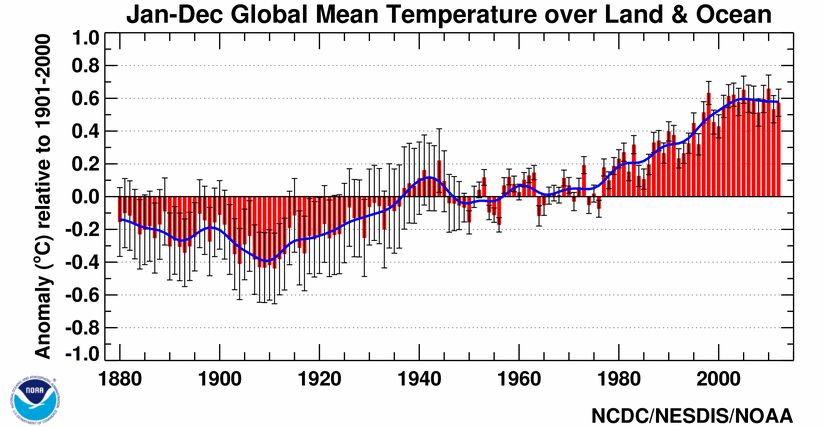
\includegraphics[scale = .5]{Figures/meantemp.png}
	\caption{Rise in Global Temperatures Since 1880 (NOAA, 2011)}
	\end{center}
\end{figure}

While there are those who contest the science, the vast majority of climatologists attribute this sustained rise in global temperatures to the increased use of fossil fuels for transportation and power. In the US, the largest source of these $CO_{2}$ emissions come from the generation of electric power followed by transportation. While no similar data could be found for the EU, Europe's lower car-utilization rate suggests that its percentage of $CO_{2}$ emisions from electric generation is higher than that of the US (global average from electric generation is roughly $\frac{1}{3}$).

\begin{figure}[H]
	\begin{center}
	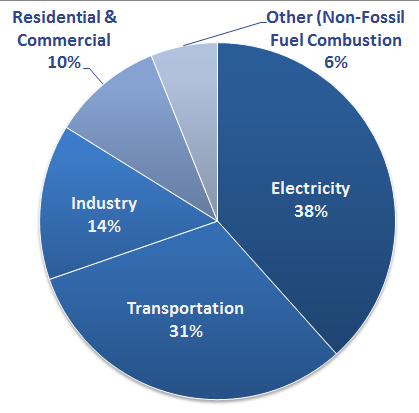
\includegraphics[scale = .5]{Figures/gases-co2.png}
	\caption{Breakdown of Greenhose Gas Emissions by Source (EPA, 2013)}
	\end{center}
\end{figure}

Clearly, if the EU, and the world, are serious about reducing greenhouse gas emissions, we will have to make changes to the way we generate electric power.

\subsection{Carbon in the EU's Political Landscape}

Currently there is no EU-wide carbon tax. In the 1990's a carbon tax was proposed to the EU Parliament, but this measure failed. However, in 2005 the EU began its emissions trading scheme (EU ETS), commonly referred to as "cap and trade". Under the EU ETS a maximum allowance of greenhouse gases (GHG) is set for each of the 11,000 plants under the regulation. If the operator emits more than its allotted amount of carbon, it is forced to buy carbon permits from other users on the market, thus constraining the aggregate emissions level (European Commission, 2013). \*

Opponents of carbon taxation argue that it is a regressive tax, since it will disproportionally hurt lower-income households. A tax on carbon would cause production costs of electricity to rise, a cost that would ultimately be passed on to the consumer. Assuming all users are charged the same rate for power, the rate increase would represent a larger share of lower-income families income. Additionally, more affluent families are able to afford the upfront capital expenditure associated with buying new, energy efficient appliances, LEED Certified homes, home solar panels, etc. while poorer household will remain reliant on electricity-produced from burning fossil fuels.

\subsubsection{Cap and Trade vs. Carbon Tax}
Theoretically, both the Cap and Trade and a carbon taxation scheme will acheive the same outcome of reducing GHG emissions, however in practice they behave quite differently. 

\begin{figure}[H]
	\begin{center}
	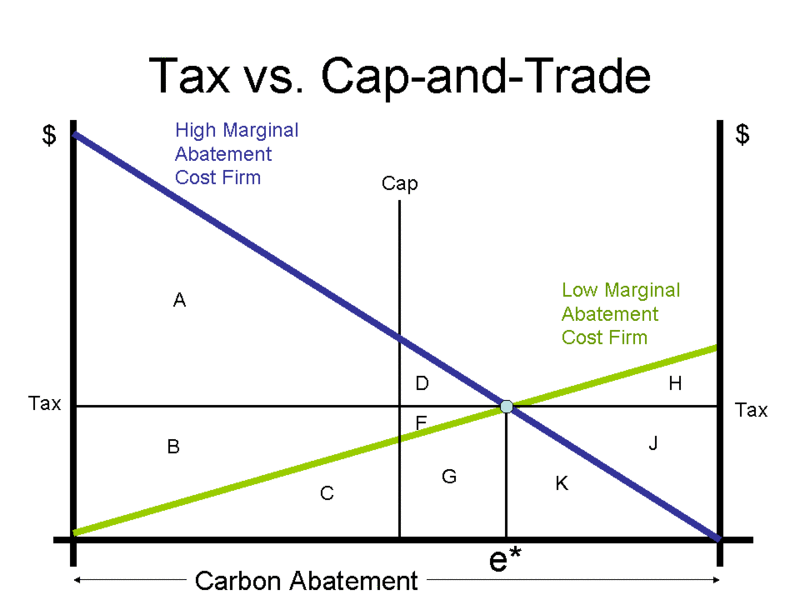
\includegraphics[scale = .4]{Figures/captrade.png}
	\caption{Carbpn Tax vs Cap and Trade (Environmental Economics)}
	\end{center}
\end{figure}


In the EU, all existing power stations were issued a base carbon allowance for free, essentially making the scheme free for them as long as they maintained current emissions levels. On the other hand, a carbon tax will impose immediate costs on all emitters as each unit of carbon has a price. This helps explain why this program was able to pass the ballot while taxation was not (Taschini, 2013). \*

Carbon taxation is more difficult to implement because the price at which it is taxed at is extreamly important-- too low and industry might just pay the tax and continue emitting GHG, too high and consumers suffer dramatically higher prices. {\bf It is this pricing problem that this paper centers on.}


\section{Carbon from Electricity}
In addition to being the largest single source of greenhouse gases, electric generation is amongst the low-hanging fruit when it comes to reducing global emissions. Chiefly this is because: 

\begin{itemize}
	\item The scale of power plants means switching one plant from coal to gas will have a large impact
	\item Power plants are designed to last 20+ years, helping capital recovery for a 'green' investment
	\item Technology is already in place for reduced or zero emission sources
	\item Even if personal transports shifts towards electric vehicles, electric generation will need to be cleaner 
\end{itemize}

Electric power demand is predicted to increase in Europe as more and more tasks traditionally fulfilled via internal combustion (IC) or natural gas (e.g. transport and home heating) become electric. This in-and-of itself is good-- large-scale electric generation is much cleaner and energy efficient than IC, however this will force governments and utility companies to build new generation stations. New power plant construction in-turn raises the question of what \emph{type} of power plants should the EU invest in. 

\subsection{The Current State of Power Generation in Europe}
Europe varies greatly when it comes to the methods used to generate electricity. Norway, produces over 90\% of their power from renewable sources, while others such as Malta produce almost 0\% of their power using renewables. Overall, the EU 27 stands at about 18\% generation from renewables. Between 1990 and 2008, the share of electricity produced from renewable sources increased by 288 TWh, an increase of 87.2\% (European Environmental Agency, 2011) 

\begin{figure}[H]
	\begin{center}
	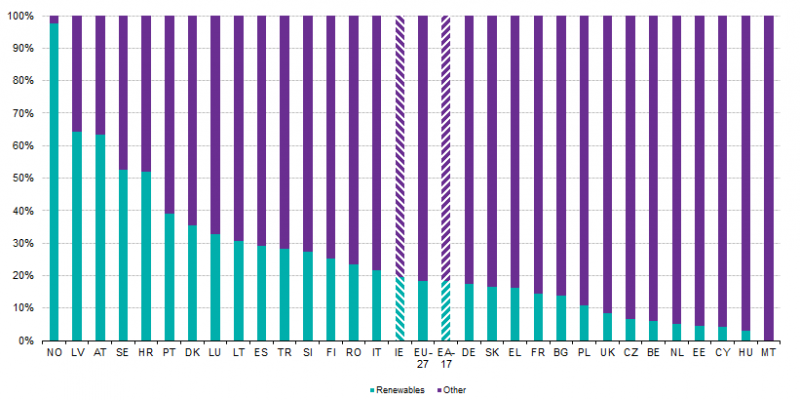
\includegraphics[scale = .6]{Figures/percentrenew.png}
	\caption{Share of Renewables in Electricity Production (Eurostat, 2012)}
	\end{center}
\end{figure}

As seen in {\bf Figure 4} for the vast majority of European nations, electric power is produced primarly by convential thermal, i.e. buring a fuel to produce heat. Traditionally this has meant coal and oil, but increasingly the world has shifted towards nuclear and natural gas as its main heat sources. As we will see, the various methods of producing this heat have dramatically different enivronmental impacts. 

\begin{figure}[H]
	\begin{center}
	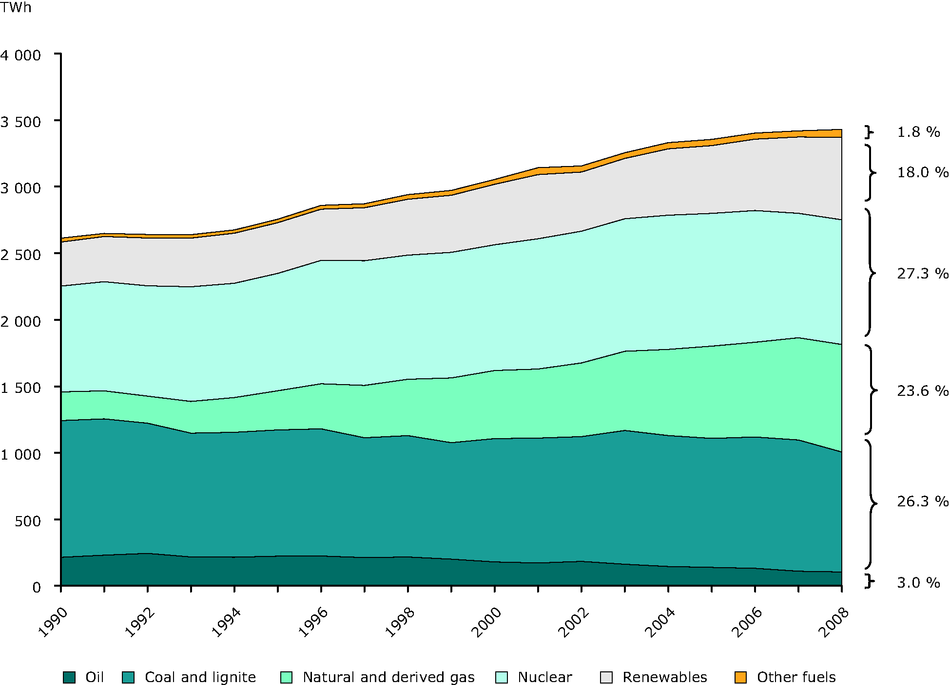
\includegraphics[scale = .4]{Figures/sourceTWh.png}
	\caption{Electric Generation by Fuel Source(Eurostat, 2012)}
	\end{center}
\end{figure}

\subsection{Methods of Generating Electricity}
All types\footnote{with the execption of fuel cells and photovoltaic which rely directly to the flow of electrons} electric generation are derivied from the same fundamental principle: Faraday's Law. Farady's Law states that a voltage is induced by a change in the magnetic environment of a coil. Electric generators operate on this principle: 1) magnets are placed along a rotating shaft 2) this shaft is placed inside to a coil of wires 3) the shaft is connected to a source of rotary motion (turbine, engine, etc.) 4) the spinning of the shaft causes a change in the magnetic field and 5) an electric voltage is produced. Fossil fuels enter the equation to provide the rotary motion. In the most general sense, some heat source (usually combustion) causes a pressure increase in steam which inturn causes a fan blade to spin. Renewable sources sidestep the combustion process and, in the case of hydroelectric and wind, use the fluid flow to turn the fan blade, or the thermal energy of the sun to heat water as in the case of solar thermal\footnote{it is important to make the disticntion between solar thermal and solar photovoltaic. The former uses solar radiation to heat a working fluid while the later exploits a property of certain materials that causes them to shift polarity when heated}\*

As mentioned earlier, the type of fuel used as the heat source dramatically effects the output of $CO_2$ and other pollutants ($NO_x$) per MWh. Reneweable sources produce zero GHG emissions, while coal and natural gas produce $CO_2$ as a byproduct of combustion. The relative emmissions are shown below:

\begin{figure}[H]
	\begin{center}
	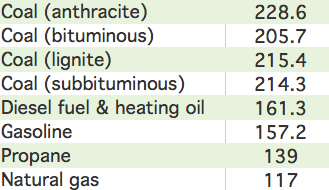
\includegraphics[scale = .5]{Figures/co2fuel.png}
	\caption{Pounds of CO2 Emitted per Million BTU(US Energy Information Administration, 2013)}
	\end{center}
\end{figure}

As seen above, natural gas produces about 57\% less $CO_2$ than bituminous coal (the most commonly used for electricity generation). Thus, it follows that replacing all existing coal power plants with natural gas would reduce GHG emissions by over half! \*

Perhaps a more striking difference than the relative $CO_2$ emissions is the cost difference between different sources. When discussing the cost per MWh, we must first establish the different factors internal to the pricing:

\begin{itemize}
\item Capital costs 
\item Fixed operations and managment 
\item Variable operations and managment (fuel)
\item Transmission investment
\item Capacity factor
\end{itemize}

The first four costs are self-explainitory, but the last is a bit subtle. The capacity factor\footnote{readers familiar with electromechanics will recognize this as the duty cycle} (CF) is the percent of time that the source will run-- a measure of intermittence. For example, if a 1 MW turbine produced 3000h MW over the course of a year, it would have a capacity factor of 34\%. Thus, a 100 MW solar installment (CF=.25) could not reliably provide as much power as a 100 MW gas turbine (CF=.87). 
More formally:

\begin{equation}
Capactiy \: Factor = \frac{Actual \: Produced}{Nominal \: Capacity}
\end{equation}

Capacity factors have large implications on the optimal energy portfolio since a certain baseload of power will be needed at all times. This suggests that a global optima of cost and emissions exists since a grid comprised completely of renewables would require a nominial capacity of three times the actual requirement-- a three-fold cost increase. {\bf This paper aims to find the Pareto optimal combination of cheap, reliable, polluting thermals with expensive, itermittent, and clean renenewables. }\*

Another important distinction is that between \emph{Dispatchable} and \emph{Non-Dispatchable}. Dispatchable technologies are those that can be switched on and off, as well as being able to ramp up or down production based on demand. Dispatchable technologies are more valuable to grid operators because they allow them the flexability to to meet the variable loads demanded throughout the day.\footnote{While techincally coal and nuclear are dispatchable, they are more traditionally used to supply base loads since they take more time (days) to ramp up. Aeroderiviative gas turbines are the ultimate dispatchable because their production can be started and stopped in a matter of hours.}

\begin{figure}[H]
	\begin{center}
	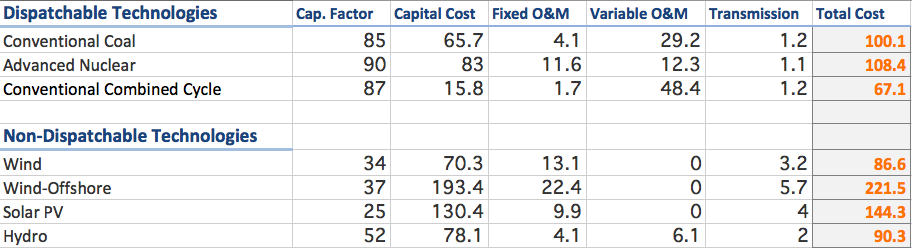
\includegraphics[scale = .5]{Figures/costssource.png}
	\caption{Levelized Costs For Various Generation Technologeis(US Energy Information Administration, 2013)}
	\end{center}
\end{figure}


\subsection{Grid Considerations}
The intermittent supply of solar and wind power raises concerns about the stability of the grid. This intermittency, coupled with the unequal demand, could cause blackouts if supply was at a low while demand was at a high (around 4pm). Conversely, if there is not enough demand to meet the supply, blackouts could be caused by wind turbines overloading the transmission lines. Transmission lines, like highways, are limited by their capacity, and large surges of energy can cause them to overload and shutdown, which can potenitally cause nationwide voltage drop and subsequent blackout (Cardwell, 2013).   



\section{Computational Model}

\subsection{Data Collection}

\subsection{Monte Carlo Simulation}

\subsection{Direchet Distribution}

\subsection{Qualification Critera}


\section{Results}

\subsection{Optimal Carbon Pricing}

\subsection{The Effect of Renewables on Consumer Utility Prices}

% \subsection{Allocation and Europe's Vulnerabilities to Adverse Supply Shocks}














\end{document}

